\documentclass[10pt]{article}

\usepackage[margin=1in]{geometry}
\usepackage{textcomp}
\usepackage{parskip}
\usepackage{amsmath}
\usepackage[backend=biber, style=alphabetic, sorting=ynt]{biblatex}
\usepackage{graphicx}
\usepackage{wrapfig}
\usepackage{float}
\usepackage{caption}

\graphicspath{{./images/}}

\addbibresource{paper.bib}

\begin{document}

\title{Developing a Bubble Chamber Particle Discriminator Using Semi-Supervised Learning}
\author{Brendon Matusch, X, Y, and Z}
\date{August 2018}
\maketitle

\begin{abstract}
    The identification of non-signal events is a major hurdle to overcome for bubble chamber dark matter experiments such as PICO-60. The current practice of manually developing a discriminator function to eliminate background events is difficult when available calibration data is frequently impure and present only in small quantities. In this study, several different input formats and neural network architectures are applied to the task. First, they are optimized in a supervised learning context. Next, two novel semi-supervised learning algorithms are trained, and found to replicate the Acoustic Parameter discriminator previously used in PICO-60 with up to 100\% accuracy.
\end{abstract}

\section{Objective}

In the PICO-60 experiment, and in most other experiments striving to directly detect dark matter, one of the most important and challenging hurdles to overcome is that of background events. Unwanted particles from a variety of sources can produce event signatures that appear very similar to those which are expected to be created by dark matter candidates.

To resolve this, physicists must determine a discriminator function that can, based on experimental data, separate events generated by possible dark matter candidates from those due to background radiation. Two general problems stand in the way:

\begin{enumerate}
    \item A detailed model of the physical environment is often used to produce an accurate discriminator. This takes a long time, and will have to be updated whenever the physical variables of the experimental apparatus change.

    \item The primary intention of many dark matter experiments, which is to reduce the number of background events to the lowest level possible, means that there will be a very small number detected. This places a significant constraint on the amount of data that is available to optimize such a discriminator.

    Furthermore, what little data is available to optimize a discriminator very often contains impurities, because whatever background radiation is present during WIMP detection runs is also present during calibration runs. These are difficult to separate without already having access to a functional discriminator, creating a ``chicken or the egg'' problem (from which a common way to escape is to create a time- and labor-intensive simulation).
\end{enumerate}

The objective of this study is to investigate the potential for machine learning techniques to address both of these issues. More specifically, in the context of the PICO-60 experiment, there are two objectives:

\begin{enumerate}
    \item Determine the most effective machine learning architecture to use in development of a discriminator. Furthermore, develop several neural network architectures and apply them to different input formats, in order to find which are the most effective.

    \item Determine whether these techniques can be extended, applying two original algorithms based on semi-supervised learning, to develop an effective discriminator function based on incomplete and inaccurate initial information.
    
    For clarity, and with specific reference to the PICO-60 experiment, the intent is to accurately separate particle types using only run types as training data. While run types are known to be mostly correlated with particle types, the relatively large percentage of impurities has the potential to hinder conventional learning techniques. Specifically, the run types available for training are:

    \begin{enumerate}
        \item Neutron calibration sets, which are known to contain approximately 90\% neutrons, and
        \item Background radiation runs, which contain approximately 99\% alpha particles
    \end{enumerate}
\end{enumerate}


The architecture described may have wider applications to several similar cases, such as those that require a discriminator which is difficult to construct using conventional techniques.

\begin{enumerate}
    \item Limited ability to collect accurate calibration data, and/or imperfect correlation between calibration data and particle types.
    \item Unknown and/or complex interactions in the experimental apparatus make a conventional discriminator difficult to define, where machine learning techniques may be able to uncover hidden correlations in the input data.
\end{enumerate}

\section{Previous PICO-60 Analysis}

\subsection{Background}

The PICO-60 bubble chamber experiment, created for the detection of weakly interacting massive particles (WIMPs) \cite{pico}, was completed in 2017. It provides an excellent basis on which to develop and test the efficacy of such techniques as a potential tool for event discrimination, relative to the conventional techniques used during initial analysis of the experiment.

WIMP candidates in the cross-section and mass ranges to which the PICO-60 detector is sensitive are predicted to produce nuclear recoils with the same properties as those induced by neutrons. The key difference is that neutrons frequently (but not always) scatter several times and produce multiple bubbles, where the extremely small predicted cross-sections of WIMP candidates mean that they should almost invariably create just one bubble. This means single-bubble neutron events can be used to optimize a discriminator to detect WIMP events.

The approximate expected ratio between single-bubble and multiple-bubble events generated by neutrons is known. A measured quantity of single-bubble events generated by nuclear recoils, in excess of this prediction, would be indicative of WIMP interactions. Consequently, it is imperative to isolate only those events associated with nuclear recoils.

\subsection{Discrimination Techniques}

\subsubsection{Overview}

In this study, newly developed methodologies were compared to the two discrimination techniques developed previously for the PICO-60 experiment: Acoustic Parameter and machine learning.

\subsubsection{Acoustic Parameter}

The Acoustic Parameter method (furthermore AP) is the technique that was used for event discrimination in the original PICO-60 analysis. A function was defined that discriminates between alpha particles and nuclear recoils based on audio data. It was derived based on a physical model of the bubble chamber, and was tuned using neutron calibration sources to produce events in the PICO-60 apparatus.

Before AP can be calculated, the audio data must first be converted into the frequency domain (specifically, with the banded Fourier transform $\beta_{8}$). It must also be preprocessed with the position correction function $PosCor(\beta_{8}, \chi)$, which adjusts the overall volume of an audio recording according to its position in the vessel. This is done because the acoustic characteristics differ significantly depending on the position of an event in the vessel.

Finally, a set of data cuts must be applied to remove certain classes of events which are not accurately classified using AP. These classes include wall event and multiple-bubble events.

These conversion, preprocessing, and data cutting steps were reapplied during this study, and are described in Section \ref{data_formats}.

\subsubsection{Machine Learning}

As part of the PICO-60 experiment, some testing was conducted to determine whether machine learning (in the form of a multi-layer perceptron) could be a viable technique to consider for a discrimination function. The results, while not definitive, indicated that the general technique warranted further investigation.

\subsection{Data Sources and Formats} \label{data_formats}

Discriminators can use a variety of different data formats to make predictions. These are collected from the two essential sensors present in the PICO-60 apparatus: piezoelectric microphones (piezos) and cameras.

\subsubsection{Piezo-Derived}

\textit{Raw Waveform}

The lowest-level data derived from the piezos is the raw waveform $\omega$. This consists of a series of samples collected every $2.5 \times 10^{-6}$ seconds. They are each represented as a 16-bit integer. Only the section of the audio between sample 90,000 (inclusive) and sample 190,000 (exclusive) was used during most experiments, because there is only background noise prior to this window, and a clipped signal produced by hydraulics repressurizing the vessel after. (These sections contain no information and can be undesirably fit on by neural networks.)

\textit{Fourier Transform}

The raw waveform $\omega$ was converted into the frequency domain by means of a one-dimensional Discrete Fourier Transform (DFT) for real input. Since DFTs produce sequences of complex numbers, the magnitude of each element was computed. The direct output from such a DFT is the full-resolution Fourier transform $\beta _{50,001}$, which consists of a sequence of numbers half the length of the raw waveform $\omega$. (It is half the length because the output of a DFT of real inputs is Hermitian, meaning there is no new information contained in the second half of the output.)

Beyond this, the banded Fourier transform $\beta_{8}$ (which is the input to the AP function and the original neural analysis) was computed by integrating the resonant energy over all frequencies within each of a set of bands. This can be thought of as a method of signal downscaling, compressing the information into a smaller number of data points.

This process was generalized to several other banding resolutions. Higher-resolution counterparts of $\beta_{8}$ included $\beta_{20}$ and $\beta_{40}$.

\begin{figure}[h]
    \centering
    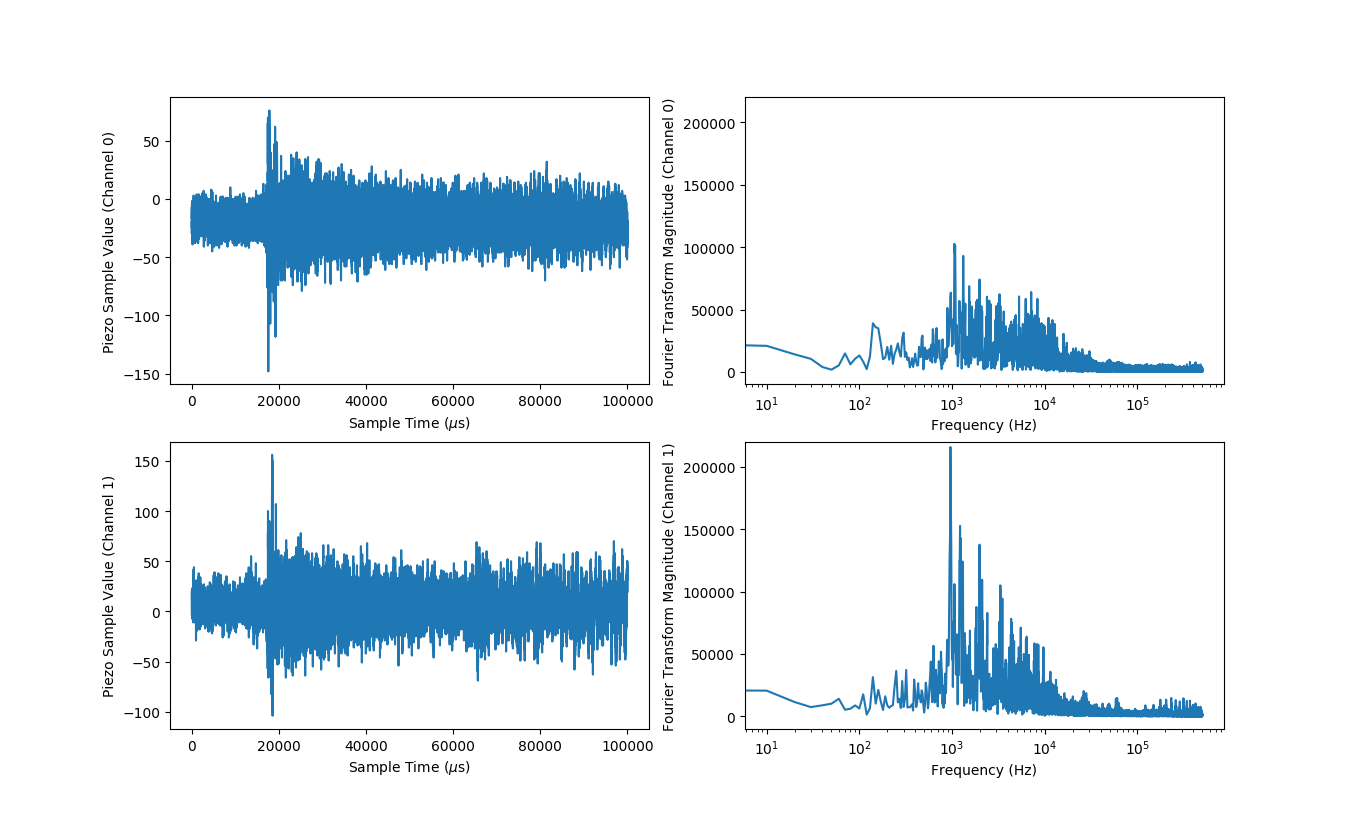
\includegraphics[width=\textwidth]{audio}
    \caption{\label{} An example of the cropped audio waveform $\omega$ and full resolution Fourier transform $\beta_{50,001}$.}
\end{figure}

\subsubsection{Camera-Derived}

\textit{Image Window Sequence}

For each event that is captured, the four cameras within the PICO-60 apparatus each capture a sequence of 71 images before and after formation of a bubble is detected using the cameras and an entropy-based trigger. These raw images contain a large amount of extraneous information; they encompass the entire vessel. To reduce the input information, the image window sequence $\iota$ includes 50\texttimes50 cropped windows around the position of the bubble. The 71 frames, many of which contain either no bubble or a bubble in later stages of formation, are reduced to 10 immediately around the formation of the bubble. Five frames from before the recording trigger are included in $\iota$, because the bubble does not cause a trigger until it is already of a significant size.

\begin{figure}[h]
    \centering
    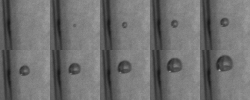
\includegraphics[width=0.7\textwidth]{image_grid}
    \caption{\label{} An example of the image sequence $\iota$.}
\end{figure}

\textit{3D Position}

The 3-dimensional position $\chi$ of the bubble within the vessel is calculated using triangulation, based on the known positions and angles of the cameras and the position of the bubble within the field of view of each camera. This is used in the banded frequency position correction function $PosCor(\beta _{8}, \chi)$, which corrects $\beta _{8}$ for variations in amplitude which depend on the position of the bubble.

\subsection{Data Cuts}

Techniques in this study are trained and validated on a number of different data sets. The selection of these sets focused on the fundamental trade-off between quality and quantity of data; by setting a higher standard for the validity of training data, one has less data to train on.

The initial data set $D$ to which these cuts are applied consists of all events recorded during PICO-60 run 2.

\subsubsection{Basic Quality Cut}

A certain number of cuts are necessarily applied to all data to ensure meaningful results. Otherwise, significant overfitting on biases in the data is likely. This basic quality cut $QualCut(D)$ consists of the following restrictions:

\begin{itemize}
    \item The run was not collected during engineering or testing
    \item Recording was triggered by the camera
    \item AP is not erroneously large and negative ($log_{10}(AP)>-100$)
    \item Recorded more than 25 seconds after reaching target pressure
    \item The bubble position $\chi$ was successfully calculated ($[\chi_{X}, \chi_{Y}, \chi_{Z}]\neq[-100, -100, -100]$)
\end{itemize}

\subsubsection{Bubble Multiplicity Cut}

PICO-60 events which include multiple bubbles are \textit{always} neutron events; alpha particles and WIMP candidates never scatter. Thus, no discriminator is required to handle these events, so they are removed. The bubble multiplicity cut $MultiCut(D)$ consists of the following restrictions:

\begin{itemize}
    \item Either 0 or 1 bubbles are detected based on images from the camera
    \item The number of bubbles approximated using the pressure transducer is close to 1
\end{itemize}

\subsubsection{Wall Cut}

Events that occur near the walls of the vessel have acoustic properties which are notably different from events nearer the center of the vessel. It can be desirable for a discriminator to handle these events correctly; however, AP does not, and neither does the neural network used in the previous PICO-60 paper. Thus, removing wall events allowed for a more meaningful direct comparison between a new neural network and existing techniques.

\begin{figure}[h!]
    \centering
    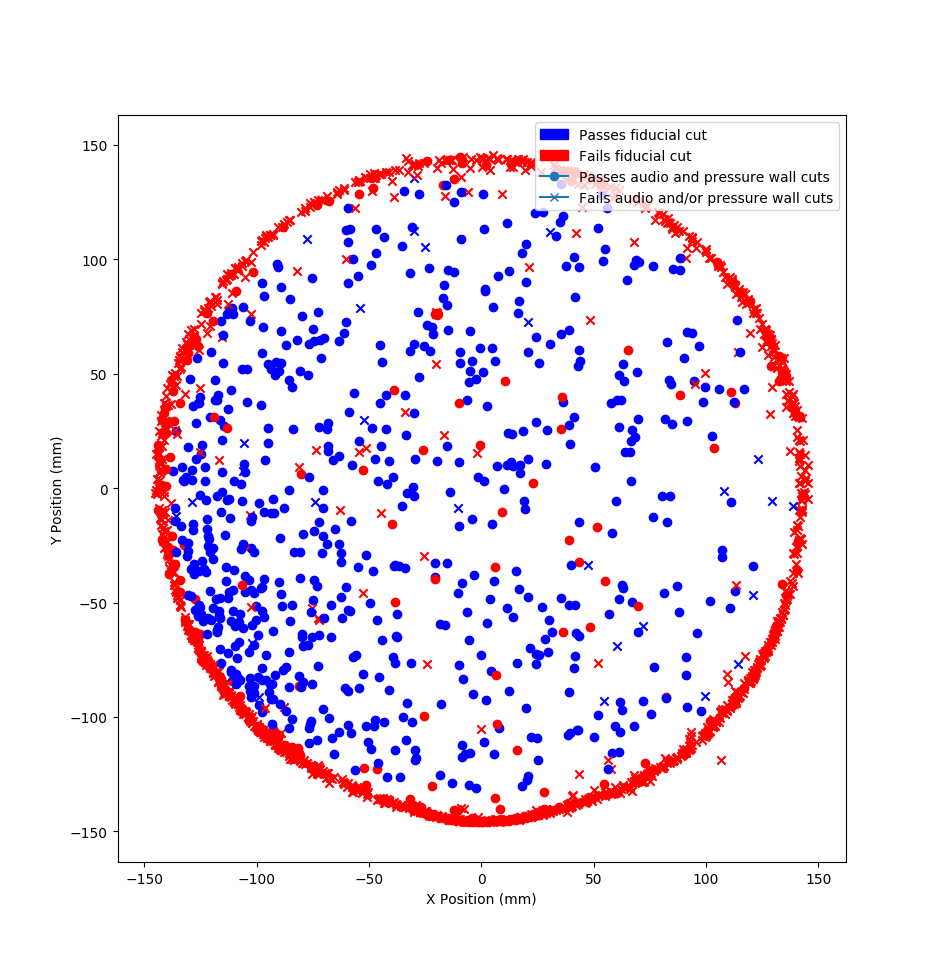
\includegraphics[width=\textwidth]{wall_event_positions}
    \caption{\label{} A visualization of the fiducial cuts and how they match up with the pressure and acoustic cuts.}
\end{figure}

The complete wall cut $WallCut(D)$ is a composition of the fiducial cut $FidWallCut(D)$ (which makes use of the 3D position $\chi$), the pressure cut $PresWallCut(D)$ (which uses data from the pressure transducer), and the acoustic cut $AcWallCut(D)$ (which uses the banded Fourier transform $\beta _{8}$). Those cuts restrict data as follows:

\begin{itemize}
    \item The fiducial cut $FidWallCut(D)$ defines a spatial area along the walls of the vessel within which no events are accepted. It determines whether events fall within this area based on the visually calculated position $\chi$.
    \item The pressure cut $PresWallCut(D)$ restricts the pressure detected by the pressure transducer, without any position corrections, to be within a range of 0.3 of 1
    \item The acoustic cut $AcWallCut(D)$ is defined using the banded Fourier transform $\beta_{8}$, and takes advantage of differences in the frequency distribution (specifically the first and second frequency bands of the first and third piezos) of wall events and non-wall events.
\end{itemize}

\section{Machine Learning Techniques}

\subsection{Background}

While machine learning has existed for many years, recent developments in artificial neural networks have opened up a wide variety of applications and fields in which it can now be used.

One of the key benefits of machine learning systems is that they have the capacity to approximate arbitrary functions (such as AP) without human intervention. This greatly alleviates the need for human programmers to define and optimize the exact algorithm used.

This characteristic has already shown wide-ranging implications in many fields. For one, it has the potential to drastically increase the speed of iteration for the people working on a project, since retraining a machine learning system when a hardware or software variable changes is much faster than calibrating a human-designed model.

\subsection{Techniques Considered}

Machine learning techniques are usually divided into two main categories:

\begin{itemize}
    \item Supervised learning, in which a system is trained on a set of fully-labeled data to classify unseen examples according to the patterns it observes in the training set, and
    \item Unsupervised learning, in which a system finds patterns or clusters in a set of unlabeled data. This can find order in almost any training set, but it is unpredictable and may not find the particular patterns desired.
\end{itemize}

A significant challenge in this application is that neither supervised nor unsupervised learning is ideal. The calibration and background runs available for training are not pure, so supervised learning is likely to overfit on biases and produce undesirable results. Conversely, unsupervised learning may be able to find clusters in the data, but it is impossible to guarantee that it will distinguish between nuclear recoils and alpha particles as opposed to some other binary separation.

For these reasons, a technique is needed that is not as sensitive to problematic training data as supervised learning, but more predictable and controllable than unsupervised learning. Semi-supervised learning is a middle ground in this regard. It makes use of a labeled set as well as an unlabeled set. It uses the labeled set for training, and uses the unlabeled set to further structure the patterns it finds in the training set (which may not be sufficiently large to apply to supervised learning).

Two original semi-supervised algorithms were developed and implemented for this study: gravitational differentiation and iterative cluster nucleation. Both are discussed in detail in Section \ref{semi_supervised}.

\subsection{Performance Analysis}

Performance of machine learning systems was evaluated using two metrics: classification accuracy and class-wise standard deviation.

Classification accuracy is the ability of the network to separate the events into the two desired classes. Numerically, this corresponds to the number of validation examples the network classifies correctly. The baseline for correctness is the run type during supervised learning experiments, and the AP prediction for semi-supervised experiments.

Class-wise standard deviation captures how decisive the network is: whether its prediction is confidently high or low, or is only slightly closer to one edge of the spectrum.

Numerically, this is a variable defined as $C$ below, where $N$ and $A$ are the sets of outputs of the supervised learning discriminator in question, corresponding to the sets of neutrons and alpha particles respectively (or calibration and background sets respectively, depending on which is used as ground truth data). It calculates the spread of the network's predictions for each ground truth class. This means that a decisive discriminator, which produces a wide separation between the two classes, is preferred over one that produces a nebulous cloud of outputs with a seemingly arbitrary decision boundary.

$S=std(N \cup A)$

$C=(std(N \div S) + std(A \div S)) \div 2$

The first step is to calculate the standard deviation $S$ of the union of $N$ and $A$. This gives an indication of the scale of the overall distribution. When $N$ and $A$ are divided by $S$, they are normalized so that the standard deviation of their union is equal to 1. While the neural network’s outputs are bounded in the range of 0 to 1 with a sigmoid activation, AP has a significantly wider range. Normalization of the union prevents this from creating a bias where AP would produce a higher standard deviation with a similarly proportioned error.

The second step is to calculate the mean of the standard deviations of the normalized sets of neutrons and alpha particles individually. This is an indication of how tightly clustered or widely dispersed the discriminator’s predictions are for each class. Very consistent predictions of $x$ for neutrons and $y$ for alphas (for any $x$ and $y$), with minimal variance off those specific values, will produce a low class-wise standard deviation.

\subsection{Optimization Process}

Each of the learning algorithms used in this study applies a neural network. For each of the general configurations (multi-layer perceptron, one-dimensional convolutional neural network, et cetera) there are many possible specific architectures with different hyperparameters, which have to be optimized to improve performance. Specific hyperparameters that were optimized include:

\begin{itemize}
    \item Number of layers of each type (dense, convolutional)
    \item Number of neurons in dense layers
    \item Number of filters in convolutional layers (depth of output tensor)
    \item Kernel size in convolutional layers (spatial area that a single filter covers)
    \item Stride in convolutional layers (spacing between kernel positions during convolution)
    \item Dropout regularization parameter (proportion of neurons to randomly remove for any given training example)
    \item L2 regularization $\lambda$ (multiplier for squared weights before adding to loss function)
\end{itemize}

Several of these hyperparameters are optimized at a time, using a grid search. Given $n$ different hyperparameters to optimize and $m$ different possible values for each, $m^n$ different networks are trained (using every possible combination of hyperparameters) and tested on a validation set.

\section{Supervised Learning}

\subsection{Overview}

The primary objective, in experimentation with supervised learning, is to determine the most effective combination of input format and neural network architecture to use in replicating a discriminator function. Three major configurations were tested:

\begin{enumerate}
    \item A convolutional neural network trained on the raw waveform $\omega$.
    \item A dense neural network trained on banded Fourier transforms $\beta_{N}$.
    \item A convolutional neural network trained on the image window data $\iota$.
\end{enumerate}

For some experimental runs, $WallCut(D)$ was not applied. This was done for 2 reasons:

\begin{enumerate}
    \item As an exploratory effort, to determine whether or not it was possible to produce an effective discriminator without wall cuts. No such attempt was made during the original PICO-60 analysis.
    \item To test the network's ability to handle complex acoustic characteristics including resonance. There is a relatively clear-cut discrimination boundary in PICO-60, but this may not be the case in other applications.
\end{enumerate}

All supervised learning configurations were trained and evaluated based on their ability to determine the origin of events: whether they are from neutron calibration source runs (predominantly neutrons) or background radiation runs (predominantly alpha particles). This metric was used for training and testing instead of AP for two reasons:

\begin{enumerate}
    \item In future experiments, when no AP equivalent is available, impure data is the only information available for training. The network structure should be selected to accommodate this.
    \item In general, supervised learning systems learn to replicate biases present in the training data set. Thus, to evaluate the network's effectiveness at processing the input data, the run type (which is used for training) must be used as a baseline instead of AP.
\end{enumerate}

\subsection{Convolutional Neural Network for Raw Waveform Analysis}

\subsubsection{Structure}

A convolutional neural network was used for analyzing the raw waveform $\omega$ directly, without any preprocessing whatsoever. This avoids any destruction of information; theoretically, a sufficiently complex neural network should be capable of deriving any characteristics needed.

For this task, a very deep (20 layers in its shallowest configuration) one-dimensional fully convolutional neural network was applied. The architecture was inspired by the M34-res network \cite{verydeepconvnets} for analysis of raw waveforms. L2 regularization was used to alleviate overfitting, and batch normalization was applied to the input to stabilize training. The network's hyperparameters were modified significantly through manual empirical testing as well as grid searches.

Two different configurations were tested:
\begin{enumerate}
    \item A configuration that operates strictly on $\omega$ with no position corrections of any kind (furthermore $DeepConv(\omega)$).
    \item A configuration with an additional position input on a lower layer such that it should be able to learn to incorporate position corrections into its outputs ($DeepConvWithPos(\omega, \chi)$). This configuration was tested both with and without $WallCut(D)$.
\end{enumerate}

\subsubsection{Results}

During early tests with variations on $DeepConv(\omega)$ without $WallCut(D)$, it was revealed to have a surprising and undesirable capacity to separate run types based on meaningless information. It was able to discriminate between events from the AmBe neutron calibration runs and events from alpha background runs with 96\% accuracy, and to separate all combined neutron calibration runs from alpha background runs with 91\% accuracy. This was determined to be caused by the network detecting and fitting on biases in the white noise at the beginning and hydraulic recompression sounds at the end of the raw waveform. This extraneous information was subsequently cropped out.

Once the audio was cropped properly, $DeepConv(\omega)$ achieved a maximum of 77\% accuracy on validation data. Using the same network architecture (except for the input layer), and still without $WallCut(D)$, $DeepConvWithPos(\omega, \chi)$ achieved 85\%. The maximum obtained on a grid search with this configuration was 91\% (although with a relatively high class-wise standard deviation of 0.61). While this is not a drastic improvement, it is a fairly strong indication that the network is able to extract meaningful information from the position, which may be used in an internal position correction of the volume.

However, there is a lack of decisiveness observed even when accuracy was relatively high, in Figure \ref{waveform_hist}. This implies that, without $WallCut(D)$, this is a suboptimal technique.

\begin{figure}[H]
    \centering
    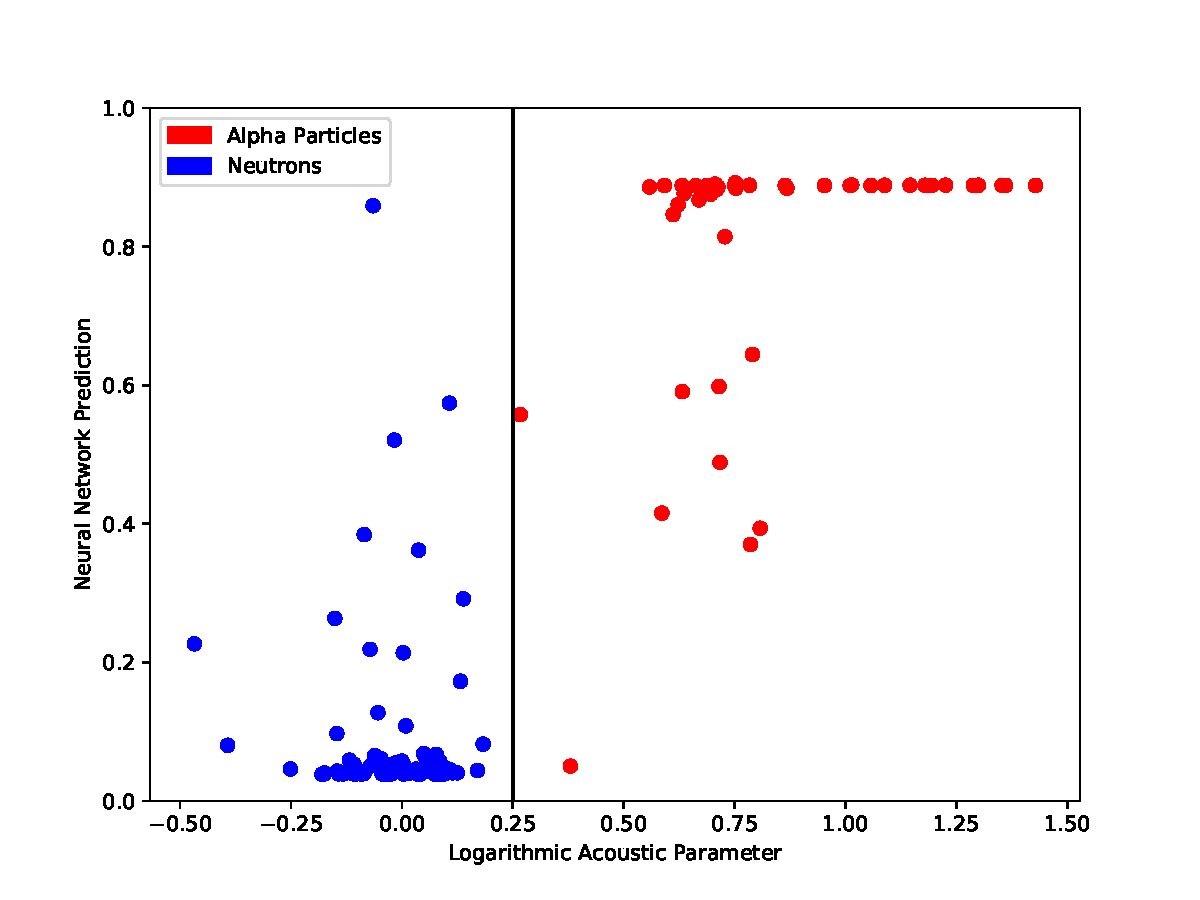
\includegraphics[width=\textwidth]{waveform_hist}
    \caption{\label{waveform_hist} Prediction distribution of the best $DeepConvWithPos(\omega, \chi)$ discriminator without $WallCut(D)$. (Validation Event Count is the number of events in the validation set that fall within a certain network prediction band.)}
\end{figure}

When $WallCut(D)$ was included, both accuracy and class-wise standard deviation improved drastically. The best configuration during a grid search was 96\% accurate and had a standard deviation of 0.41 (seen in Figure \ref{waveform_wall_cut_hist}). This is better by both metrics than the multi-layer perceptron used in the original PICO-60 analysis.

\begin{figure}[H]
    \centering
    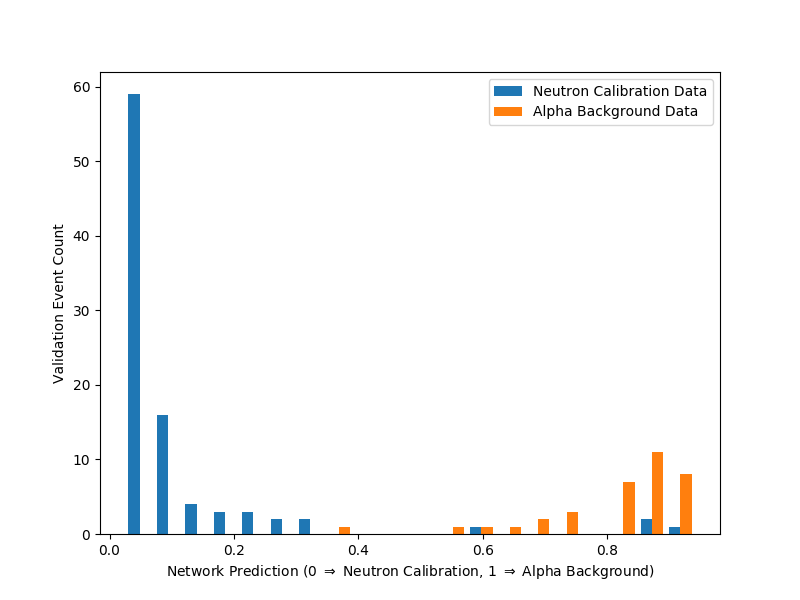
\includegraphics[width=\textwidth]{waveform_wall_cut_hist}
    \caption{\label{waveform_wall_cut_hist} Prediction distribution of the best $DeepConvWithPos(\omega, \chi)$ discriminator with $WallCut(D)$.}
\end{figure}

The following tables show the results of several $DeepConvWithPos(\omega, \chi)$ discriminators produced throughout testing, with corresponding network hyperparameters.

\begin{center}
    \captionof{table}{$DeepConvWithPos(\omega, \chi)$ with $WallCut(D)$.}
    \begin{tabular}{|l|l|l|l|l|l|l|}
        \hline
        L2 $\lambda$ & Dropout & Filters & Kernel Size & \# Layers Multiplier & Max Accuracy & Class-Wise Std Dev \\
        \hline
        0.003 & 0 & 24 & 3 & 3 & 95\% & 0.44 \\
        \hline
        0.003 & 0 & 48 & 5 & 3 & 96\% & 0.41 \\
        \hline
        0.003 & 0.5 & 24 & 5 & 3 & 93\% & 0.50 \\
        \hline
        0.001 & 0 & 48 & 5 & 3 & 95\% & 0.48 \\
        \hline
        0.001 & 0.25 & 48 & 3 & 6 & 93\% & 0.62 \\
        \hline
        0.0003 & 0.5 & 24 & 5 & 6 & 95\% & 0.49 \\
        \hline
    \end{tabular}

    \captionof{table}{$DeepConvWithPos(\omega, \chi)$ without $WallCut(D)$.}
    \begin{tabular}{|l|l|l|l|l|l|l|}
        \hline
        L2 $\lambda$ & Dropout & Filters & Kernel Size & \# Layers Multiplier & Max Accuracy & Class-Wise Std Dev \\
        \hline
        0.003 & 0 & 24 & 3 & 3 & 91\% & 0.61 \\
        \hline
        0.003 & 0.5 & 24 & 5 & 3 & 91\% & 0.65 \\
        \hline
        0.001 & 0.25 & 24 & 3 & 3 & 91\% & 0.66 \\
        \hline
        0.001 & 0.5 & 48 & 5 & 3 & 88\% & 0.73 \\
        \hline
        0.0003 & 0 & 48 & 5 & 6 & 78\% & 0.95 \\
        \hline
        0.0003 & 0.5 & 48 & 5 & 6 & 74\% & 0.92 \\
        \hline
    \end{tabular}
\end{center}

These tables show that, both with and without $WallCut(D)$, simple network architectures seem to produce better accuracy, likely due to reduced overfitting. Larger kernel sizes, more filters, and more layers make performance generally worse, while higher L2 regularization does the opposite. Dropout seems to have a weak correlation, possibly reducing accuracy slightly.

\subsection{Multi-Layer Perceptron for Fourier Transform Analysis}

\subsubsection{Structure}

Preprocessing the audio by applying a Fourier transform may be advantageous. If the frequency distribution and overall volume are indeed the most important factors for discrimination, the network can gather them straight from the Fourier transform $\beta_{N}$ rather than having to analyze $\omega$ to extract this information.

In addition to the Fourier transform used in the original PICO-60 analysis, higher resolutions were computed by similar means. These included $\beta _{20}$ and $\beta _{40}$. Also, the full-resolution $\beta _{50,001}$ was input into a neural network directly, without any downscaling.

$WallCut(D)$ was applied to the low-resolution Fourier transforms during early experiments (since they were used for AP) to minimize the number of variables between initial neural networks and a proven discriminator.

Once again, configurations with and without position input were tested. This time, position corrections were optionally included when position input was not used. The resulting configurations are furthermore referred to as $FourierMLP(\beta_{N})$, $FourierMLP(PosCor(\beta_{N}, \chi))$ and $FourierMLPWithPos(\beta_{N}, \chi)$. Several different resolutions $N$ of $\beta_{N}$ were used. While a variety of network architectures were tested, most had a small number of layers (on the order of three), applied dropout and L2 regularization, and used batch normalization once again.

\subsubsection{Results}

It became evident very quickly that, without $WallCut(D)$, a high resolution was not required to get a high accuracy relative to the ground truth data. $FourierMLP(\beta_{8})$ managed an excellent 98\% validation accuracy, and also produced a mean class-wise standard deviation of 0.29. Its very decisive prediction distribution can be observed in Figure \ref{banded_no_pos_input_hist}. Increasing the number of bands to $FourierMLPWithPos(beta_{20}, \chi)$, did not improve the results; accuracy only reached 95\%, with an increased mean standard deviation of 0.42. Using 40 bands reduced the accuracy once again, to 91\%.

\begin{figure}[H]
    \centering
    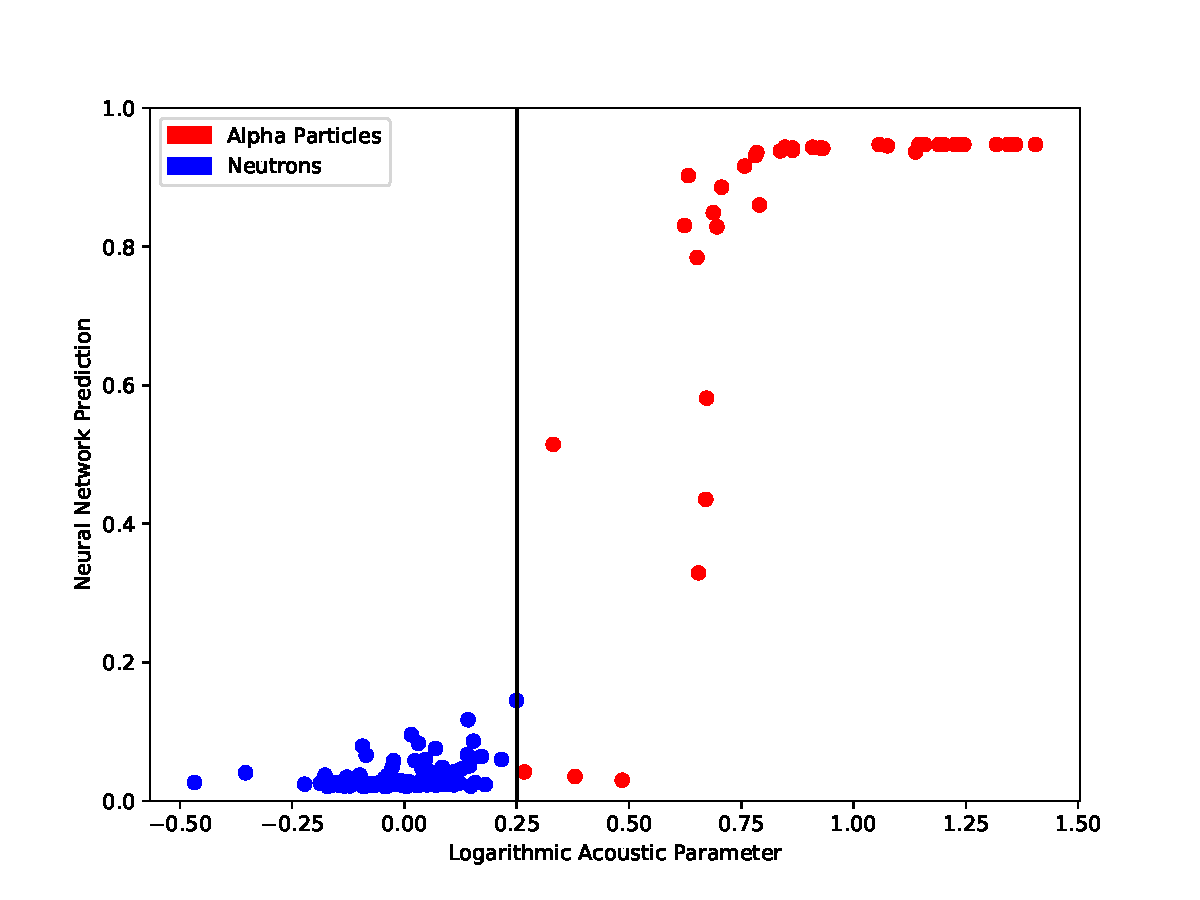
\includegraphics[width=\textwidth]{banded_no_pos_input_hist}
    \caption{\label{banded_no_pos_input_hist} Prediction distribution of the best $FourierMLP(\beta_{8})$ discriminator, with $WallCut(D)$.}
\end{figure}

Very interestingly, $FourierMLP(\beta_{8})$ performed better than either $FourierMLP(PosCor(\beta_{8}), \chi)$ or \\ $FourierMLPWithPos(\beta{8}, \chi)$, which produced accuracy values of 97\% and 95\%, respectively.

Unlike for the convolutional neural network trained on $\omega$, position input did not improve performance at all. In fact, $FourierMLP(\beta_{8})$, performed better than $FourierMLPWithPos(\beta_{8}, \chi)$, which reached only 95\% validation accuracy. Nevertheless, they both performed better than any of the network architectures trained on $\omega$.

The higher resolution demonstrated significant power when $WallCut(D)$ was not applied, and only \\ $QualCut(MultiCut(D))$ was used. $FourierMLPWithPos(\beta_{20}, \chi)$ achieved only 92\% accuracy (2 percentage points lower than the same configuration without $WallCut(D)$). However, training on $\beta_{50,001}$, which does not incorporate any banding, improved this figure to a maximum of 97\%. However, that epoch had a relatively high class-wise standard deviation, at 0.47, as seen in Figure \ref{high_freq_no_wall_hist}.

\begin{figure}[H]
    \centering
    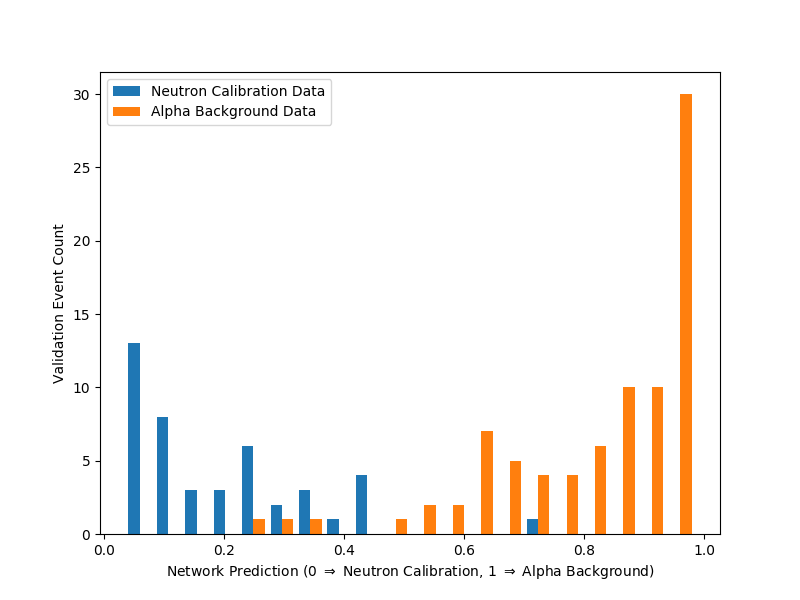
\includegraphics[width=\textwidth]{high_freq_no_wall_hist}
    \caption{\label{high_freq_no_wall_hist} Prediction distribution of the best $FourierMLPWithPos(\beta_{50,001}, \chi)$ discriminator, without $WallCut(D)$.}
\end{figure}

The following tables compare various multi-layer perceptron discriminators, with and without wall cuts.

\begin{minipage}{\textwidth}
    \begin{center}
        \captionof{table}{Neural networks trained on Fourier transforms with $WallCut(D)$.} \label{fft_wall_cuts}
        \begin{tabular}{|l|l|l|l|l|l|}
            \hline
            Configuration & L2 $\lambda$ & Dropout & Layers & Max Accuracy & Class-Wise Std Dev \\
            \hline
            $FourierMLP(PosCor(\beta_{8}))$ & 0 & 0.5 & 2 & 95\% & 0.56 \\
            \hline
            $FourierMLP(\beta_{8})$ & 0 & 0.5 & 2 & 98\% & 0.29 \\
            \hline
            $FourierMLPWithPos(\beta_{8}, \chi)$ & 0 & 0.5 & 3 & 95\% & 0.44 \\
            \hline
            $FourierMLPWithPos(\beta_{8}, \chi)$ & 0 & 0.25 & 3 & 97\% & 0.43 \\
            \hline
            $FourierMLPWithPos(\beta_{20}, \chi)$ & 0.003 & 0.25 & 3 & 93\% & 0.54 \\
            \hline
            $FourierMLPWithPos(\beta_{20}, \chi)$ & 0 & 0 & 3 & 94\% & 0.52 \\
            \hline
            $FourierMLPWithPos(\beta_{40}, \chi)$ & 0 & 0 & 3 & 91\% & 0.57 \\
            \hline
            $FourierMLPWithPos(\beta_{50,001}, \chi)$ & 0.0003 & 0 & 4 & 91\% & 0.53 \\
            \hline
            $FourierMLPWithPos(\beta_{50,001}, \chi)$ & 0.001 & 0.25 & 4 & 91\% & 0.56 \\
            \hline
            $FourierMLPWithPos(\beta_{50,001}, \chi)$ & 0.001 & 0.5 & 3 & 89\% & 0.64 \\
            \hline
            $FourierMLPWithPos(\beta_{50,001}, \chi)$ & 0.01 & 0.5 & 4 & 89\% & 0.65 \\
            \hline
        \end{tabular}
    \end{center}
\end{minipage}

\begin{minipage}{\textwidth}
    \begin{center}
        \captionof{table}{$FourierMLPWithPos(\beta{N})$ trained without $WallCut(D)$.}
        \begin{tabular}{|l|l|l|l|l|l|}
            \hline
            Configuration & L2 $\lambda$ & Dropout & Layers & Max Accuracy & Class-Wise Std Dev \\
            \hline
            $FourierMLPWithPos(\beta_{20}, \chi)$ & 0 & 0 & 3 & 92\% & 0.63 \\
            \hline
            $FourierMLPWithPos(\beta_{50,001}, \chi)$ & 0 & 0 & 3 & 95\% & 0.49 \\
            \hline
            $FourierMLPWithPos(\beta_{50,001}, \chi)$ & 0.001 & 0 & 2 & 96\% & 0.47 \\
            \hline
            $FourierMLPWithPos(\beta_{50,001}, \chi)$ & 0.01 & 0 & 2 & 97\% & 0.47 \\
            \hline
            $FourierMLPWithPos(\beta_{50,001}, \chi)$ & 0.01 & 0.25 & 2 & 95\% & 0.54 \\
            \hline
            $FourierMLPWithPos(\beta_{50,001}, \chi)$ & 0.01 & 0.5 & 2 & 94\% & 0.53 \\
            \hline
        \end{tabular}
    \end{center}
\end{minipage}

It is very clear in Table \ref{fft_wall_cuts} that higher resolutions do not improve accuracy. Regularization, both dropout and L2, appears to have relatively little effect.

Without wall cuts, the full-resolution Fourier transform produces much more effective discriminators. Here, L2 regularization is beneficial, possibly because there is more noise that can be overfit on.

\subsection{Convolutional Neural Network for Image Window Analysis}

\subsubsection{Structure}

It is an open question whether or not there is any information in the image data $\iota$ that could be used to distinguish between particle classes. Relative to the extremely short period of time in which the bubble forms (on the scale of nanoseconds), the framerate of the camera (340Hz) is extremely slow. While the very early stages of bubble formation (when the sound is produced) are known to differ depending on whether the bubble was created by a nuclear recoil or an alpha particle, it is unknown whether any visually apparent differences persist when the bubble is visible.

In an effort to resolve this, a two-dimensional convolutional neural network was applied to the task of discriminating based on $\iota$. The network architecture consists of a moderate number of convolutional layers (on the scale of nine) and three dense layers at the end. L2 regularization was used on all layers, and dropout was additionally used on the dense layers. No position input is used (since there are no microphones that would require position correction), so the basic configuration is $ImageConv(\iota)$.

\subsubsection{Results}

Throughout a variety of different network architectures, the best validation accuracy obtained was a deceptively high 85\%. The corresponding training accuracy of 100\% indicates that severe overfitting is taking place (not unexpected, given the relatively small image data set). Also, the class-wise standard deviation was a very high 0.95, which implies its decisions are nearly random (as seen in Figure \ref{image_hist}). It is likely fitting on some form of noise within $\iota$. The fact that throughout many trials (including a grid search), no good performance on validation data was observed, provides significant evidence that images provide insufficient information for effective discrimination.

\begin{figure}[h]
    \centering
    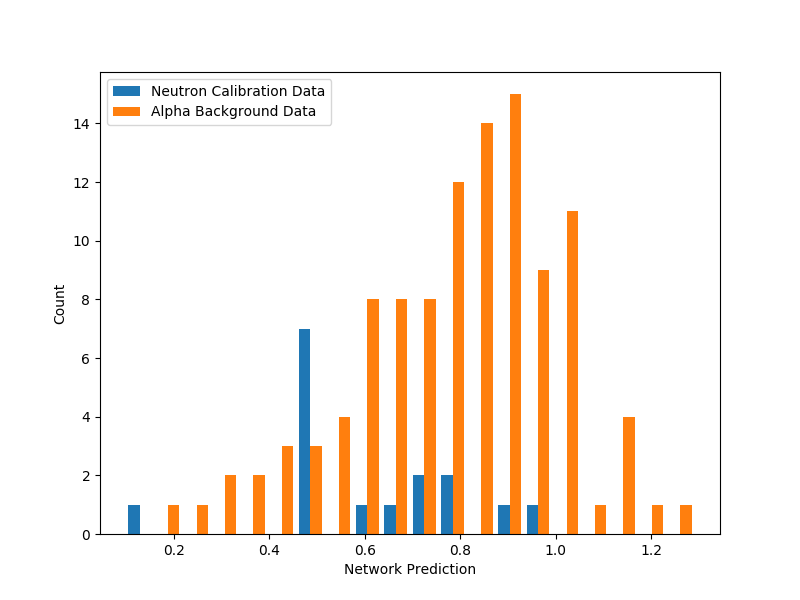
\includegraphics[width=\textwidth]{image_hist}
    \caption{\label{image_hist} Prediction distribution of the best $ImageConv(\iota)$ discriminator.}
\end{figure}

\begin{center}
    \captionof{table}{Performance of $ImageConv(\iota)$ configurations, trained without $WallCut(D)$.}
    \begin{tabular}{|l|l|l|l|l|l|}
        \hline
        L2 $\lambda$ & Dropout & Convolutional Layers & Dense Layers & Max Accuracy & Class-Wise Std Dev \\
        \hline
        0 & 0.5 & 4 & 3 & 77\% & 1.01 \\
        \hline
        0 & 0.25 & 4 & 3 & 85\% & 0.95 \\
        \hline
        0.01 & 0.25 & 4 & 3 & 66\% & 0.97 \\
        \hline
        0.003 & 0.25 & 4 & 3 & 69\% & 0.97 \\
        \hline
        0.01 & 0.25 & 12 & 3 & 66\% & 0.98 \\
        \hline
        0.01 & 0.5 & 12 & 3 & 68\% & 0.99 \\
        \hline
    \end{tabular}
\end{center}

The high standard deviations across the board are further evidence for the hypothesis that there is insufficient information in the image data.

\subsection{Performance Summary}

The following tables compare the accuracy and mean class-wise standard deviation values of certain highlight supervised learning configurations with multiple input formats, with the original PICO-60 neural network provided as a baseline.

\begin{minipage}{\textwidth}
    \begin{center}
        \captionof{table}{Summary of supervised learning configurations, trained with $WallCut(D)$.}
        \begin{tabular}{|l|l|l|}
            \hline
            Configuration & Max Accuracy & Mean Class-Wise Standard Deviation \\
            \hline
            $FourierMLP(PosCor(\beta_{8}), \chi)$ & 97\% & 0.42 \\
            \hline
            $FourierMLP(\beta_{8})$ & 98\% & 0.29 \\
            \hline
            $FourierMLPWithPos(\beta_{8}, \chi)$ & 95\% & 0.44 \\
            \hline
            $FourierMLPWithPos(\beta_{20}, \chi)$ & 94\% & 0.52 \\
            \hline
            $FourierMLPWithPos(\beta_{40}, \chi)$ & 91\% & 0.54 \\
            \hline
            $FourierMLPWithPos(\beta_{50,001}, \chi)$ & 91\% & 0.53 \\
            \hline
            Original PICO-60 Neural Network & 94\% & 0.99 \\
            \hline
        \end{tabular}
    \end{center}
\end{minipage}

\begin{minipage}{\textwidth}
    \begin{center}
        \captionof{table}{Summary of supervised learning configurations, trained without $WallCut(D)$.}
        \begin{tabular}{|l|l|l|}
            \hline
            Configuration & Max Accuracy & Mean Class-Wise Standard Deviation \\
            \hline
            $FourierMLPWithPos(\beta_{20}, \chi)$ & 92\% & 0.63 \\
            \hline
            $FourierMLPWithPos(\beta_{50,001}, \chi)$ & 97\% & 0.47 \\
            \hline
            $DeepConv(\omega)$ & 77\% & 0.86 \\
            \hline
            $DeepConvWithPos(\omega, \chi)$ & 91\% & 0.61 \\
            \hline
            $ImageConv(\iota)$ & 85\% & 0.95 \\
            \hline
        \end{tabular}
    \end{center}
\end{minipage}

There are 2 key conclusions to be drawn from the above tables:

\begin{enumerate}
    \item With $WallCut(D)$, the low-resolution Fourier transform $\beta_{8}$ is by far the most effective input format. Higher resolutions seem to make performance worse, likely due to overfitting. It is significantly better than the original PICO-60 neural network, and is more decisive (as measured by the class-wise standard deviation)
    \item Without $WallCut(D)$, full-resolution $\beta_{50,001}$ is the most effective, nearing the best performance with wall cuts at separating run types. All models are notably less decisive, given that the lowest standard deviation without wall cuts is 0.47, compared to 0.29 with wall cuts.
\end{enumerate}

Based on these results, experimentation with semi-supervised learning proceeded using \\ $FourierMLP(PosCor(\beta_{8}))$, applying a 3-layer perceptron architecture, and using $WallCut(D)$. There were three main reasons for this:

\begin{enumerate}
    \item This was a highly effective configuration with wall cuts, producing 97\% accuracy and a class-wise standard deviation dramatically better than the original PICO-60 neural network on that data set.
    \item The use of the exact same input format as AP makes the algorithms more directly comparable.
\end{enumerate}

\section{Semi-Supervised Learning} \label{semi_supervised}

\subsection{Overview}

Semi-supervised learning is an uncommon machine learning technique, relative to widely-used supervised and unsupervised learning. The concept is to train a machine learning model on a set of labeled (classified) data in addition to a set of unlabeled (unclassified) data.

In the context of PICO-60, the labeled sets consist of the neutron calibration runs, and the background radiation runs (which consist predominantly of alpha particles). In general, these labeled sets should have a strong but not perfect correlation with particle types. The unlabeled data can consist of any mixture of particle types.

The primary advantage of semi-supervised learning is clear: it requires fewer labels to be collected than conventional supervised learning. A less obvious but powerful secondary advantage is that, since the learning process allows the network to reinforce its own decisions, the negative effect of impure training data is minimized, potentially allowing the resulting network to perform better than a network trained with supervised learning.

Two techniques for semi-supervised learning have been developed for this study: gravitational differentiation and iterative cluster nucleation. The essence of both algorithms is a positive feedback loop. First, the network is trained on a smaller amount of imperfect data. Throughout the training process, the network runs predictions on unlabeled data. By using its most confident predictions in the training process, the desired function (separating particle types) is continuously reinforced, while less confident predictions are de-emphasized. This effectively draws new, unlabeled data into the training set.

Since the intent of these techniques is to separate particle types (the same as AP), performance evaluations (accuracy and class-wise standard deviation) use AP as a baseline. Note that $WallCut(D)$ was once again applied for semi-supervised learning, because $FourierMLP(PosCor(\beta_{8}))$ was used for a neural network configuration, and because AP requires application of $WallCut(D)$ to be meaningfully comparable to any neural network.

\subsection{Gravitational Differentiation}

\subsubsection{Concept}

Gravitational differentiation is a novel technique, developed during this study, for training a neural network in a semi-supervised fashion on a relatively small set of imperfectly labeled data, while simultaneously incorporating the network's changing predictions on a set of unlabeled data to encourage decisive classifications.

In general terms, it amplifies the training effect associated with high-confidence predictions (those that most clearly show characteristics of either an alpha particle or a neutron) on unlabeled examples. Meanwhile, it minimizes the training impact of low-confidence predictions, such that the network will not be trained to make incorrect predictions.

Analogous to a gravitational effect, events with high-confidence predictions are attracted closer to their corresponding classifications. They are then used as training data, allowing the patterns they represent to be used more generally to make predictions on other events.

The system accomplishes this using a new method for calculating gradients for the last layer of the neural network. Based on the current predictions of a trained network on a certain unlabeled training example, a gradient is calculated for the last layer with the following purposes:

\begin{itemize}
    \item For examples with confident predictions close to 0 or 1: Create a large gradient that pulls the prediction closer to 0 or 1 through gradient descent (like gravity).
    \item For examples with low-confidence predictions close to 0.5: Create a gradient near 0 that does not affect training significantly.
\end{itemize}

The gradients produced by this technique are used for training in the same way as gradients calculated with a loss function. Backpropagation is used to calculate gradients for previous layers, and a stochastic gradient descent optimizer is used for weight updates.

\subsubsection{Algorithm}

Gradients are calculated using the gravitational differentiation function $GravDiff(p, \psi, g)$, which is parameterized by the network's existing prediction $p$ on the training example in question, the degree $\psi$ of the piecewise exponential function used to distort the response of the gradient, and the gravitational multiplier $g$. The function is defined as follows:

$GravDiff(p, \psi, g) = g \cdot sgn(p) \cdot abs(tanh(2(p - 0.5))) ^ \psi$

It is a distortion of the hyperbolic tangent that flattens the central range and comparatively exaggerates the asymptote on either side. The equation above can be described in the following steps:

\begin{enumerate}
    \item Transform the network's prediction $p$, so its range is 1 to -1 rather than 0 to 1.
    \item Apply the sigmoidal hyperbolic tangent, producing a value of 0 in the center and asymptotic slopes to -1 and 1 at the edges.
    \item \label{exponent} What is really desired is a shallow slope in the center (so low-confidence network outputs near 0.5 will produce very shallow output gradients). Apply a relatively large exponent which is $\psi$ (in the range of 3 to 11) to squash values close to 0 closer to 0.
\end{enumerate}

(Note that step \ref{exponent} only works if $p$ is an odd integer (because odd integer exponents preserve the sign), limiting the ability to fine-tune this function by changing $\psi$. To resolve this, a piecewise exponential function is used instead, where the absolute value is taken prior to applying the power and the sign is multiplied back in afterwards. This permits use of the full range of curves produced by even and non-integer values of $\psi$.)

\begin{figure}[H]
    \centering
    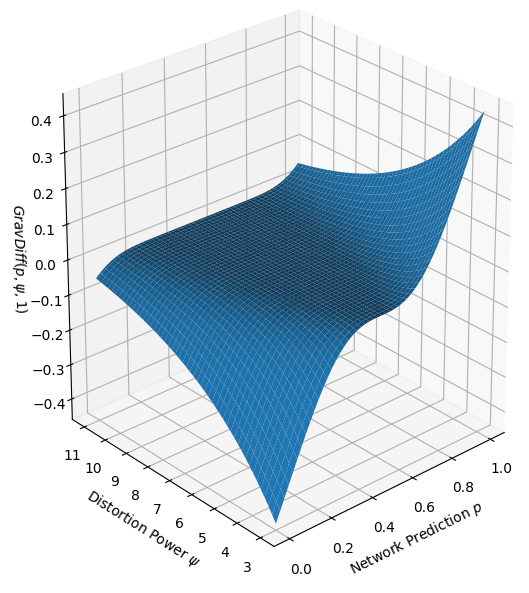
\includegraphics[width=0.8\textwidth]{grav_diff}
    \caption{\label{grav_diff} A visualization of $GravDiff(p, \psi, g)$ with respect to $p$ and $\psi$.}
\end{figure}

\subsubsection{Application}

This function is applied in a training algorithm that is parameterized by the set of imperfectly labeled data $\varsigma$, the set of unlabeled training data $\upsilon$, a binary classification neural network $NN(x)$ (where $x$ is the input data format), and the gravitational multiplier increment $\delta_g$. The distortion power $\psi$ is assumed to be constant throughout a training run, and the gravitational multiplier $g$ is initialized at 0, gradually increasing during training. It iterates as follows:

\begin{enumerate}
    \item Train $NN(x)$ for a single epoch on the combined set $\varsigma \cup \upsilon$, using the predefined ground truths for $\varsigma$ (with a mean squared error loss function) and the most recently calculated gravitational gradients for each of the examples in $\upsilon$.
    \item Calculate predictions $p$ with $NN(x)$ on the entirety of $\upsilon$. Calculate $GravDiff(p, \psi, g)$ and record the resulting gradients for the next iteration.
    \item Increment $g$ by $\delta_{g}$. At the beginning, when $g = 0$, training will be entirely based on the labeled set $\varsigma$, and progressively, over the course of a run, the gravitational effect increases with $g$.
\end{enumerate}

This system was trained using a multi-layer perceptron with an 8-band Fourier transform input for $NN(x)$, because this was one of the most successful configurations in supervised learning. It produced the highest accuracy as well as the lowest class-wise standard deviation.

\subsubsection{Results}

During a grid search of parameters of the gravitational differentiation algorithm (in addition to the stochastic gradient descent learning rate), the algorithm achieved a maximum of 98\% validation accuracy. The mean over that run (also the highest overall) was 96\%. Figure \ref{grav_grid_search} shows the highly accurate replication of AP.

As seen in Figure \ref{grav_acc_by_hyper}, all three hyperparameters that were optimized during the grid search had a significant effect on accuracy:

\begin{itemize}
    \item Smaller gravitational multipliers improved performance; the best value tested was 0.0005. This implies that the gravity effect on each unlabeled event should be weighted lightly compared to the labeled examples.
    \item Higher learning rates improve performance, with the best value tested at a quite high 0.03.
    \item Larger distortion powers (which raise the confidence threshold for a significant gravitational effect) improved performance, with the best tested at 11.
\end{itemize}

Two different options were tested with regard to size of the labeled data set $\varsigma$. Out of a set of 496 total examples available for training, either 128 (approximately $1/4$ of the total set) or 256 (approximately $1/2$) were used as labeled data. Over the entire grid search, runs with 128 examples in $\varsigma$ produced on average 64\% more errors on validation data, compared to those with 256 examples.

!!!Include table on grid search!!!

\begin{figure}[H]
    \centering
    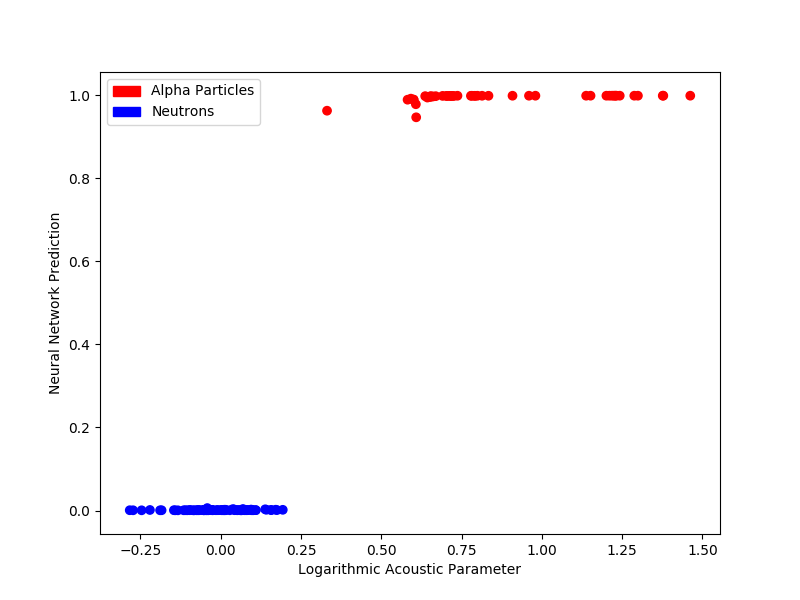
\includegraphics[width=\textwidth]{grav_grid_search}
    \caption{\label{grav_grid_search} Accuracy of best gravitational differentiation training run compared to AP (98\% accuracy).}
\end{figure}

\begin{figure}[H]
    \centering
    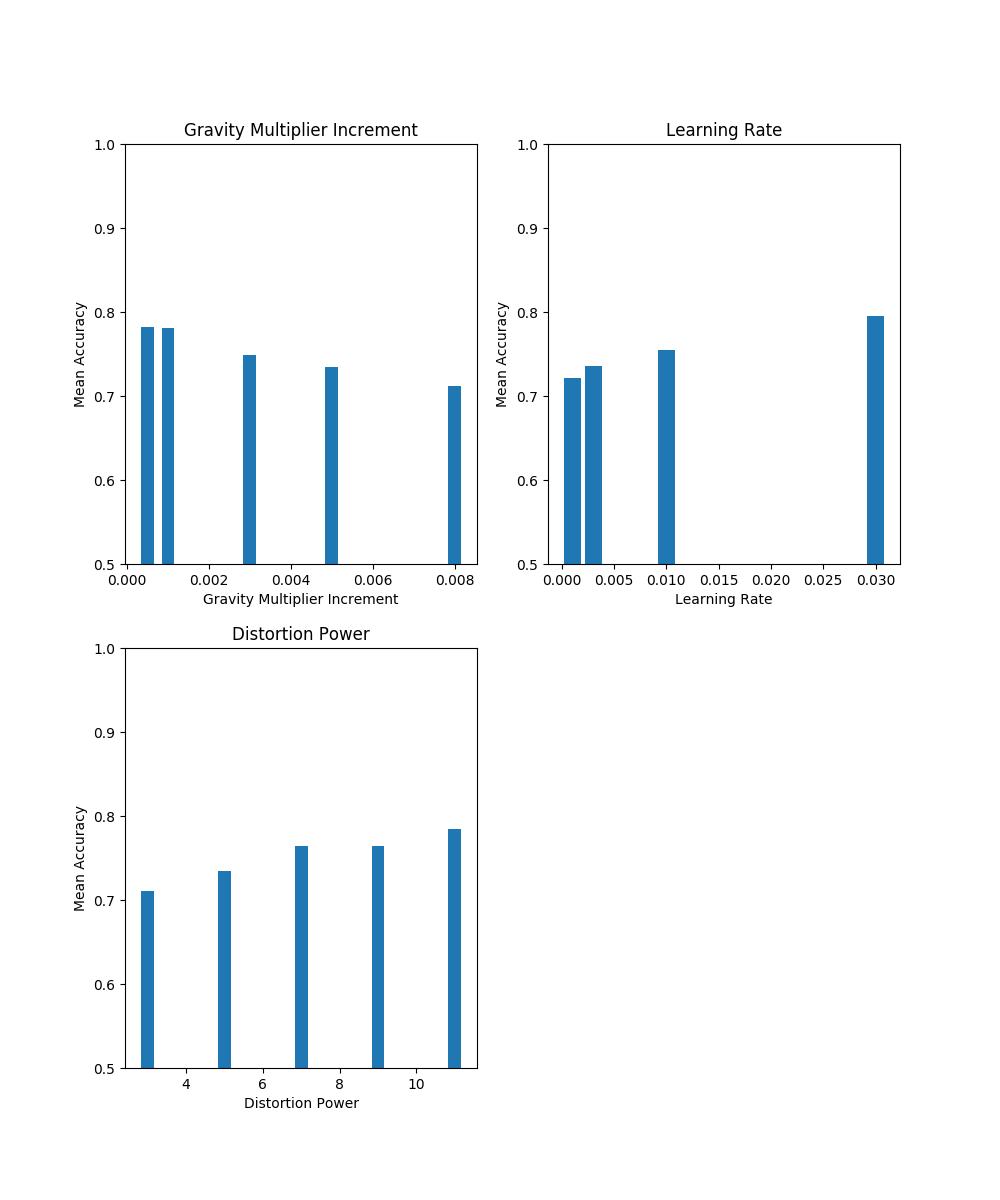
\includegraphics[width=\textwidth]{grav_acc_by_hyper}
    \caption{\label{grav_acc_by_hyper} Accuracy of gravitational differentiation as a function of hyperparameter values.}
\end{figure}

\subsection{Iterative Cluster Nucleation}

\subsubsection{Concept}

Iterative cluster nucleation is a second original semi-supervised learning algorithm developed as part of this study. It takes advantage of some amount of imperfectly labeled data, using it to classify the rest of an unlabeled training set while optimizing to produce an effective discriminator.

The basic concept is similar to that of gravitational differentiation. Starting with a relatively small amount of labeled data from two classes (nuclear recoils and alpha particles, in this case), predictions are run on a set of unlabeled data, and those predictions are used to produce further training data. However, there are two key differences:

\begin{enumerate}
    \item In iterative cluster nucleation, an unlabeled example is not included in the training process at all, until a very confident prediction is made on it. Once that occurs, it is added to the training set, expanding one of the two ``clusters'' of training data.
    \item Once an example is added to the active training set, it is never removed. This ensures that the highly confident predictions made at the very beginning continue to influence the training process.
    \item The unlabeled examples, once added to the active training set, are weighted just as strongly as examples from the original labeled data set. This ensures imperfect labels in the labeled data do not outweigh the confident and more likely correct predictions from later in the training process.
\end{enumerate}

\subsubsection{Algorithm}

The algorithm is initialized as follows:

\begin{enumerate}
    \item Take a subset of the training data, referred to as the seed set $\varsigma$. Use this as the beginning of the training set.
    \item Remove classifications from any other available training examples. These create the unlabeled set $\upsilon$.
    \item Compile and randomly initialize the weights of a binary classification neural network $NN(x)$.
\end{enumerate}

Parameterized by the initial seed threshold $j$ (on the order of 0.01) and the seed threshold multiplier $k$ (on the order of 1.05), the algorithm follows these iterative steps:

\begin{enumerate}
    \item Train $NN(x)$ for 30 epochs on $\varsigma$, using the imperfect ground truth values available.
    \item Using the partially trained weights of $NN(x)$, run inference on the entirety of $\upsilon$, producing a set of predictions $p$.
    \item Find predictions within $p$ that are within a distance of $j$ of either 0 or 1; as this is a binary classifier, such a prediction represents high confidence. Remove any such examples from $\upsilon$ and add them to $\varsigma$. The principle is that, when $NN(x)$ is trained on a relatively small set for short period of time, the few predictions within $p$ that are very confident are highly likely to be correct.
    \item If no examples have been removed from $\upsilon$ and added to $\varsigma$, multiply $j$ by $k$ in place. This is done to increase the acceptance rate later in the training process, when most easily classifiable examples have been added to $\varsigma$. Otherwise, gridlock would occur, where certain examples could not be confidently classified given the training set.
\end{enumerate}

\subsubsection{Results}

During a grid search of these parameters (in addition to regularization parameters of the network), the best accuracy achieved for replication of AP was exactly 100\%. The mean of all epochs within that training run was 98\%.

As seen in Figure \ref{icn_grid_search}, the network learned to replicate AP very accurately. Interestingly, the examples with AP values between the neutron and alpha particle ranges were also classified as such by the network. This may imply the indecisiveness on these examples is fundamental to the data rather than an implementation problem with AP.

\begin{figure}[h]
    \centering
    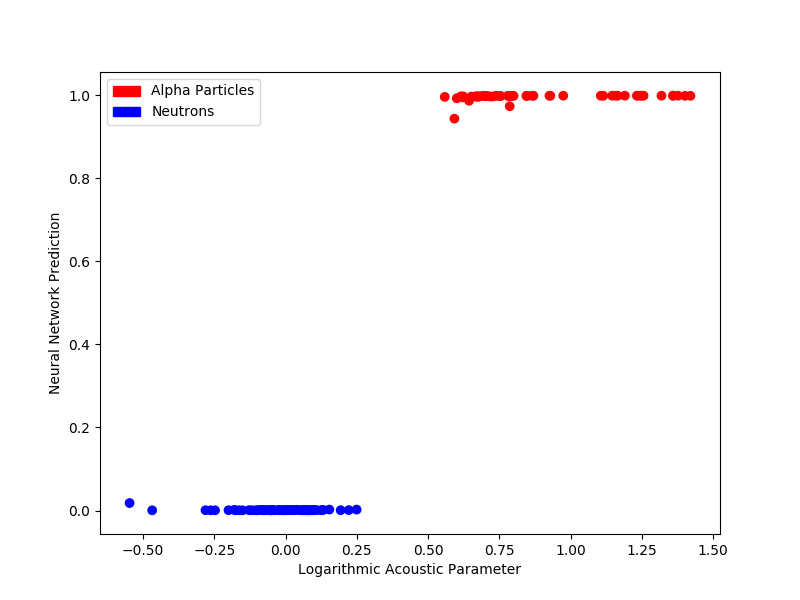
\includegraphics[width=\textwidth]{icn_grid_search}
    \caption{\label{icn_grid_search} Accuracy of optimal iterative cluster nucleation training run compared to AP (100\% accuracy).}
\end{figure}

Digging deeper into the performance throughout the runs of the grid search, Figure \ref{icn_acc_by_hyper} shows the mean accuracy as a function of each of the hyperparameters that were optimized. Dropout has a clear effect, with 25\% shown to be the optimal number of neurons to drop. L2 regularization is also significant; all $\lambda$ values greater than 0 make performance worse.

Compared to gravitational differentiation, there is a larger delta between the number of errors on the validation set depending on the number of initial training examples used. Those with 128 examples in $\varsigma$ make 85\% more errors on average. However, iterative cluster nucleation with 128 examples still makes 19\% fewer errors than gravitational differentiation with 256 examples in $\varsigma$.

\begin{figure}[H]
    \centering
    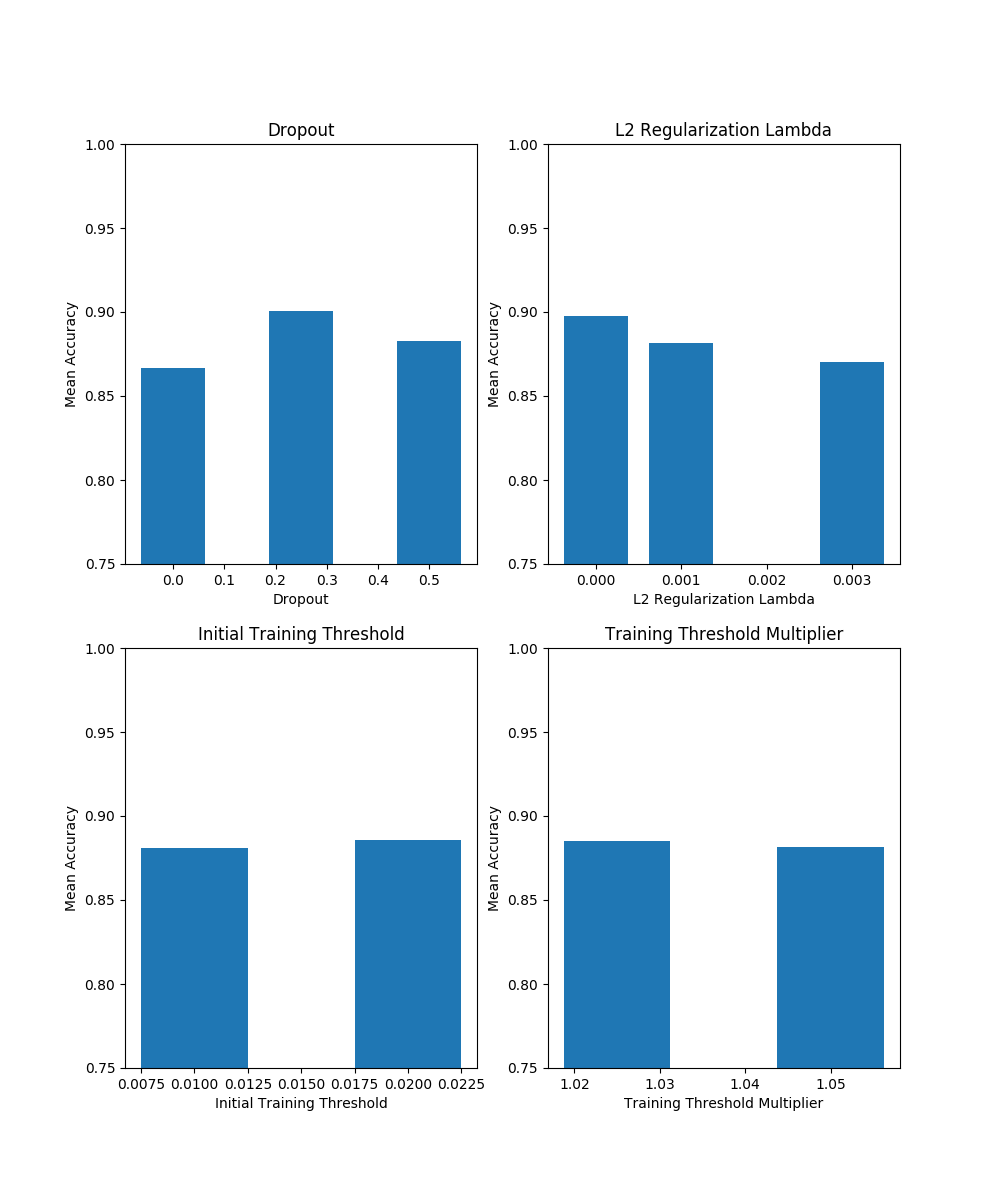
\includegraphics[width=\textwidth]{icn_acc_by_hyper}
    \caption{\label{icn_acc_by_hyper} Mean accuracy of iterative cluster nucleation as a function of hyperparameter values.}
\end{figure}

\subsection{Performance Summary}

The following table directly compares performance of the semi-supervised learning systems, with the existing PICO-60 neural network provided as a baseline once again. Note that ``Max AP Accuracy'' refers to accuracy at replication of AP, rather than replication of the ground truths.

\begin{tabular}{|l|l|l|l|}
    \hline
    Technique & Max AP Accuracy & Max Mean by Run & Class-Wise SD \\
    \hline
    Gravitational Differentiation (256 $\varsigma$) & 98\% & 96\% & TODO \\
    \hline
    Gravitational Differentiation (128 $\varsigma$) & TODO & TODO & TODO \\
    \hline
    Iterative Cluster Nucleation (256 $\varsigma$) & 100\% & 98\% & TODO \\
    \hline
    Iterative Cluster Nucleation (128 $\varsigma$) & TODO & TODO & TODO \\
    \hline
    Existing NN TODO & X & X & X \\
    \hline
    AP TODO & X & X & X \\
    \hline
\end{tabular}

\section{Conclusions}

This study has demonstrated that it is possible, using semi-supervised learning, to automatically optimize a discriminator with performance comparable to one developed and tuned by humans like the Acoustic Parameter technique. This conclusion has been achieved through two rounds of optimization, the first to explore and evaluate various network structures and input formats using supervised learning, and the second to incorporate the most successful configuration into semi-supervised learning systems with the goal of replicating AP as accurately as possible.

In the realm of supervised learning, it was made clear that the banded Fourier transform is the most effective input format. It produced significantly higher accuracy and tighter prediction distributions than neural networks trained on either the raw audio waveform or image window data. There is strong evidence that image data in particular does not contain sufficient information to be used for discrimination.

Two semi-supervised learning algorithms were developed, applying the best configuration found for supervised learning. While both techniques produced some very effective discriminators, iterative cluster nucleation was found to be the more effective of the two. It replicated AP with a mean of 98\% accuracy on the best configuration. This indicates that the technique shows significant promise.

While there is still of course a place for conventionally developed discriminators such as AP, they are difficult to develop until a large quantity of calibration data has been collected and the physical principles of the experiment are understood well. The innovations developed in this study suggest that semi-supervised learning can facilitate very quick development of discriminators immediately after the first calibration runs are conducted on a new experimental apparatus. This has the potential to allow the teams working on these experiments to iterate more quickly and better understand intermediate results, before all data has been analyzed in depth.

\section{Technologies}

All programming for this study was done in Python 3. Keras \cite{keras}, running on a TensorFlow backend, was used for all machine learning tasks. NumPy and SciPy were used for linear algebra and signal processing. ROOT, scikit-image and scikit-learn were used for data loading and storage. Matplotlib was used for data visualization.

\printbibliography

\end{document}
